\documentclass{report}
\usepackage{amsmath}
\usepackage{libertine}
\usepackage{tikz}
\usetikzlibrary{intersections}
\usetikzlibrary{through}
\begin{document}

$
r_{\!_{11}} = -r\cos(\theta -\alpha) + \sqrt{\strut R_1^2 - r^2\sin^2(\theta - \alpha)}
$
\\
\\
$
r_{\!_{12}} = R_1 \cos \alpha - r\cos(\theta - \alpha)  + \\ ~ \qquad \sqrt{\strut [R_1 \cos \alpha - r\cos(\theta-\alpha) ]^2 - r^2\sin^2 \theta - [R_1 - r\cos \theta]^2 + R_2^2}
$
\\
\begin{align*}
\rho(r,\theta) &=  \int_{-\alpha_2}^{\alpha_1} f_{\alpha}(\alpha) \int_{r_{\!_{11}}}^{\infty} f_l(l)dl d\alpha +  \int^{2\pi-\alpha_2}_{\alpha_1} f_{\alpha}(\alpha) \int_{r_{\!_{12}}}^{\infty} f_l(l)dl d\alpha  \\
&=\int_{-\alpha_2}^{\alpha_1} \frac{1}{2\pi} e^{-\lambda \pi r_{\!_{11}}^2} d\alpha +  \int^{2\pi-\alpha_2}_{\alpha_1} \frac{1}{2\pi} e^{-\lambda \pi r_{\!_{12}}^2} d\alpha
\end{align*}
\\
\begin{tikzpicture}
	\draw (-1.5,0) -- (1.5,0);
	\draw (0,-1.5) -- (0,1.5);
	\draw (0,0) circle [radius=1cm];
\end{tikzpicture}
\\
\begin{tikzpicture}[scale=0.05]
	\coordinate [label=left:{\small $BS$}] (A) at (0,0);
	\fill [red,opacity=.5] (A) circle (50pt);
	
	\coordinate [label=right:{\small $U$}] (B) at (150,0);
	\fill [green,opacity=.5] (B) circle (50pt);
	
	\coordinate [label=above:{\small $R$}] (C) at (125,50);
	\fill [blue,opacity=.5] (C) circle (50pt);

	\draw (A) -- node[below=2pt] {\small $r_0$} (B) -- node[right=2pt] {\small $r_2$} (C)
	-- node[above=2pt] {\small $r_1$} cycle;
	
\end{tikzpicture}
\\
$
\text{policy:} \{r_1 < r_0, r_2 < \big(\frac{P_a}{P_b}\big)^{\frac{1}{\alpha}}r_0\}
$
\\
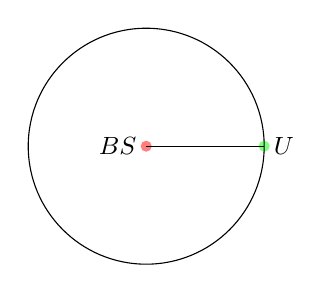
\begin{tikzpicture}[scale=0.01]
	\coordinate [label=left:{\small $BS$}] (A) at (0,0);
	\coordinate [label=right:{\small $U$}] (B) at (150,0);
	\fill [red,opacity=.5] (A) circle (200pt);
	\fill [green,opacity=.5] (B) circle (200pt);

	\draw (A) -- (B);
	\node (D) [name path=D,draw,circle through=(B)] at (A) {};
\end{tikzpicture}
\\
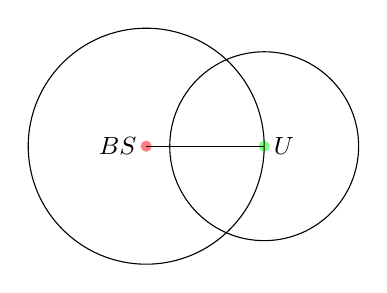
\begin{tikzpicture}[scale=0.01]
	\coordinate [label=left:{\small $BS$}] (A) at (0,0);
	\coordinate [label=right:{\small $U$}] (B) at (150,0);
	\fill [red,opacity=.5] (A) circle (200pt);
	\fill [green,opacity=.5] (B) circle (200pt);

	\draw (A) -- (B);
	\node (D) [name path=D,draw,circle through=(B)] at (A) {};
%	\node (E) [name path=E,draw,circle(60)] at (B);
	% Name the coordinates, but do not draw anything:
	\draw (B) circle(120);
\end{tikzpicture}
\\
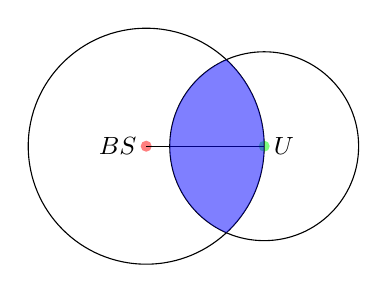
\begin{tikzpicture}[scale=0.01]
	\coordinate [label=left:{\small $BS$}] (A) at (0,0);
	\coordinate [label=right:{\small $U$}] (B) at (150,0);
	\fill [red,opacity=.5] (A) circle (200pt);
	\fill [green,opacity=.5] (B) circle (200pt);

	\draw (A) -- (B);
	\node (D) [name path=D,draw,circle through=(B)] at (A) {};
%	\node (E) [name path=E,draw,circle(60)] at (B);
	% Name the coordinates, but do not draw anything:
	\draw (B) circle(120);
	\begin{scope}
		\clip (0,0) circle(150);
		\fill[blue,opacity=.5] (150,0) circle (120);
	\end{scope}
	%	\path [name intersections={of=D and E}];

\end{tikzpicture}
\end{document}

